\documentclass[../Main.tex]{subfiles}
\begin{document}
\chapter{Deep Learning}

\intro{
    The modern term “deep learning” goes beyond the neuroscientific perspectiv on the current breed of machine
    learning models. It appeals to a more general principle of learning multiple levels of composition,
    which can be applied in machine learning frameworks that are not necessarily neurally inspired.
}

\begin{figure}[H]
    \centering
    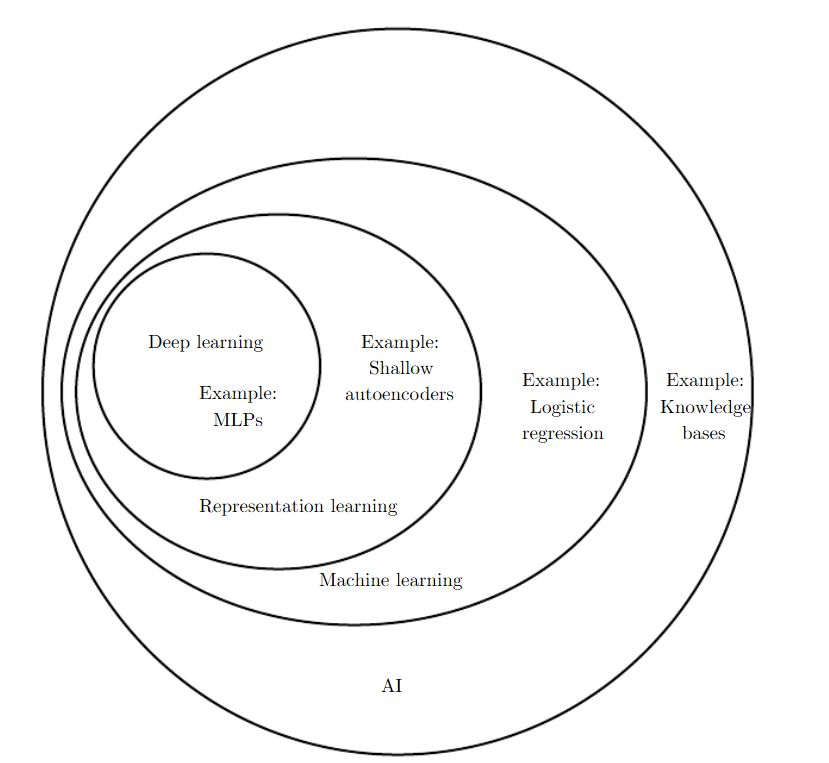
\includegraphics[width=0.75\linewidth]{Images/deepl-venn.png}
    \caption{A Venn diagram showing how deep learning is a kind of representation learning, which is in turn a kind of machine learning, 
    which is used for many but not all approaches to AI. Each section of the Venn diagram includes an example of an AI technology}
\end{figure}

\section{Differences to standard statistical learning methods}
\begin{enumerate}
    \item No manual feature extraction
    \item Arbitarily Complex Models
    \item No Feature Engineering
    \item Flexible Models
\end{enumerate}

\subsection{Reasons for increasing popularity}
\begin{itemize}
    \item Bigger datasets due to increasing digitalization
    \item Increasing Model Sizes due to more computational resources
    \item Many more (see trends like transformers)
\end{itemize}

\newpage
\section{Short Linear Algebra Recap}

\begin{figure}[H]
    \centering
    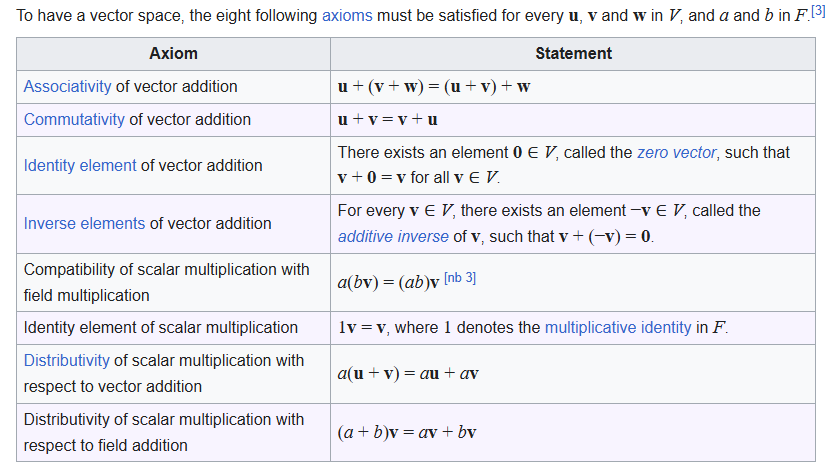
\includegraphics[width=0.75\linewidth]{Images/vector-space.png}
    \caption{Rules of a vector space}
\end{figure}

\begin{multicols}{2}
    Ein Skalar ist eine mathematische Größe,
    die allein durch die Angabe eines Zahlenwertes
    charakterisiert ist (in der Physik gegebenenfalls mit Einheit).
    \begin{equation}
        \text{Scalar} = s = 2
    \end{equation}

    \begin{equation}
        \text{Matrix} = \textbf{A} =
        \begin{bmatrix}
            1 & 2 & 3\\
            a & b & c
        \end{bmatrix} = \mathbb{R}^{2 \times 3}
    \end{equation}

    \begin{equation}
        \text{Vector} = \textbf{b} =
        \begin{bmatrix}
            1 \\
            a
        \end{bmatrix} = \mathbb{R}^2
    \end{equation}

    \begin{equation}
        \text{Tensor} = \mathbb{R}^{n_1 \times n_2 \times n_i}
    \end{equation}

    \begin{equation}
        \boldsymbol{I}_3 =
        \begin{bmatrix}
            1 & 0 & 0 \\
            0 & 1 & 0 \\
            0 & 0 & 1
        \end{bmatrix}
    \end{equation}
    The identity matrix can be thought of 
    as the matrix version of the number 1.
\end{multicols}

\defn{Diagonal Matrices}{
    \begin{equation}
        \begin{split}
            diag(\boldsymbol{v}) \Rightarrow D_{i,j} &= 0, \forall i \neq j \\
            diag(\boldsymbol{v}) \boldsymbol{x} &= \boldsymbol{v} \odot \boldsymbol{x} \\
            I_n &= diag(\boldsymbol{v})
        \end{split}
    \end{equation}

    Inverting diagonal matrices is 
    only possible, if all diagonal 
    elements are non-zero.
    \begin{equation}
        diag(v)^{-1} = diag([1/v_1, \cdots, 1/v_n]^T)
    \end{equation}

    \begin{itemize}
        \item Many generic machine learning 
        algorithms can be simplified by 
        restricting some matrices to be 
        diagonal matrices
    \end{itemize}
}

\defn{Symmetric Matrix}{
    Is a matrix that is equal to its transpose:
    \begin{equation}
        \boldsymbol{A} = \boldsymbol{A}^T
    \end{equation}
    \begin{equation*}
        \begin{bmatrix}
            1 & 1 & -1 \\
            1 & 2 & 0 \\
            -1 & 0 & 5
        \end{bmatrix}
    \end{equation*}
}

\defn{Orthonormal}{
    Ortho means that angle between the 
    vectors is a 90° angle and normal 
    means that the length of the vector is 
    one.
    In \(\mathbb{R}^n\), there are at most n such 
    vectors, which have a non-zero norm.
    \begin{equation}
        \begin{split}
            \boldsymbol{x}^T \boldsymbol{y} &= 0 \\
            ||\boldsymbol{x}||_2 &= 1
        \end{split}
    \end{equation}
}

\defn{Orthogonal Matrix}{
    An orthogonal matrix (should be 
    called an orthonormal matrix), is 
    a square matrix whose rows are 
    mutually orthonormal and whose 
    columns are mutually 
    orthonormal.

    \begin{equation}
        \boldsymbol{A}^T \boldsymbol{A} = \boldsymbol{A}^T = \boldsymbol{A}
    \end{equation}

    The the inverse is simply the transpose:
    \begin{equation}
        \boldsymbol{A}^{-1} = \boldsymbol{A}^T
    \end{equation}
}

\subsection{Products}

\defn{Dot Product}{
    \begin{equation}
        \boldsymbol{a} \cdot \boldsymbol{b} = \sum_{i} a_i b_i
    \end{equation}

    \begin{equation}
        \boldsymbol{x}^T \cdot \boldsymbol{y} = ||x||_2 ||y||_2 cos \theta
    \end{equation}
}

\defn{Matrix Product}{
    The matrix product C=AB is simply a matrix where \(C_{i,j}\) 
    is the dot product between row i of A and column j of B.
    \begin{equation}
        \begin{split}
            \boldsymbol{C} &= \boldsymbol{A} \boldsymbol{B} \neq \boldsymbol{B} \boldsymbol{A} \\
            C_{i,j} &= \sum_k A_{i,k} B_{k,j} \\
            A(B+C) &= AB + AC \\
            A(BC) &= (AB)C
        \end{split}
    \end{equation}
}

\defn{Hadamard Prod}{
    Is the element-wise product:
    \begin{equation}
        C = A \odot B
    \end{equation}
}

\begin{figure}[H]
    \centering
    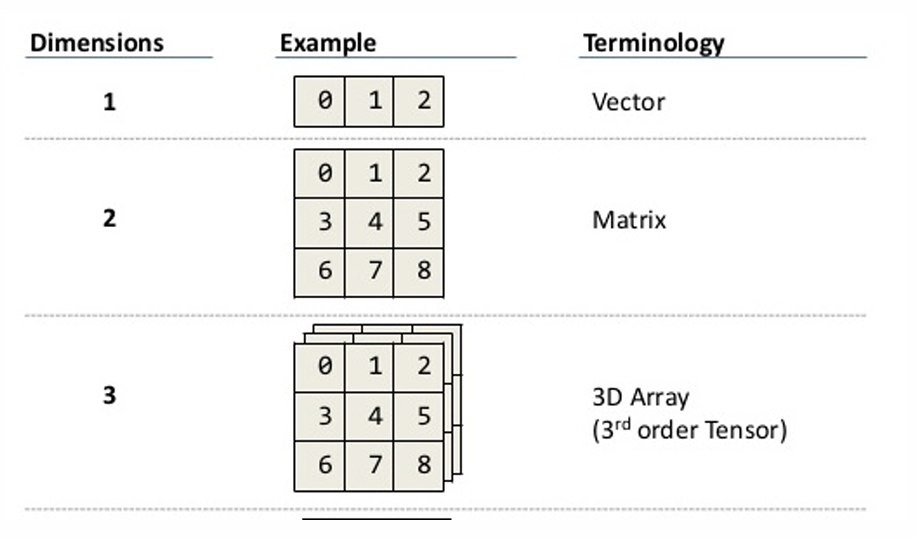
\includegraphics[width=0.75\linewidth]{Images/terminology-linalg.png}
    \caption{Linear Algebra Terminology}
\end{figure}

\defn{Multiplicative inverse}{
    Is a number which when multiplied by x yields the multiplicative identity, 1.
    In linear algebra we define an inverse matrix:
    \begin{equation}
        \boldsymbol{A}^{-1} \boldsymbol{A} = \boldsymbol{I}_n
    \end{equation}
}

\subsection{Solving Systems}
\defn{Lineare Gleichungssysteme}{
    Linear system of equations in its most compact form:
    \begin{equation}
        \boldsymbol{A} x = b \\
        A \in \mathbb{R}^{m \times n} \\
        b \in \mathbb{R}^m
    \end{equation}
    Oder auch anders geschrieben:
    \begin{equation}
        \begin{split}
            A_{1,1} x_1 + \cdots + A_{1,n} x_n &= b_1 \\
            \vdots & \\
            A_{m,1} x_1 + \cdots + A_{m,n} x_n &= b_m
        \end{split}
    \end{equation}

    Mit analytischer Lösung:
    \begin{equation}
        x = \boldsymbol{A}^{-1}b
    \end{equation}

   \begin{itemize}
    \item Mit Anzahl Lösungen:
    \begin{itemize}
        \item Keine, 1, Oder unendlich viele
    \end{itemize}
    \item  Note that using the inverse might 
            numerically not be the best approach.
 
    \item Requiring A to have the same or 
        more rows (n) than columns (m) 
        is a necessary condition for Ax=b 
        to have a unique solution.
        It is though not sufficient, since 
        the rows might be redundant.

    \item We need at least m 
        linearly independent column 
        vectors in A this will allow the 
        column space to cover \(\mathbb{R}^m\)

    \item If we want Ax=b to have at most one 
    solution, we require 
    that there are at most m columns. 
    Otherwise, there is more than one 
    way of parameterizing each solution
    Hence for \(A^{-1}\) to exist, we require 
    m=n, where all the columns are linearly independent
   \end{itemize}
}

\defn{Span}{
    A matrix contains column vectors 
    \(A_{:,i}\) , hence Ax can be interpreted 
    as a linear combination of these vectors.
    It can be imagined as a vector 
    pointing from the origin into space 
    and hence Ax is the weighted 
    concatenation of these vectors.

    \begin{equation}
        \boldsymbol{Ax} = \sum_i x_i \boldsymbol{A}_{:,i}
    \end{equation}

    The span of a set of vectors is now 
    defined as the set of all points 
    obtainable by linear combinations of 
    these vectors.
}

\begin{figure}[H]
    \centering
    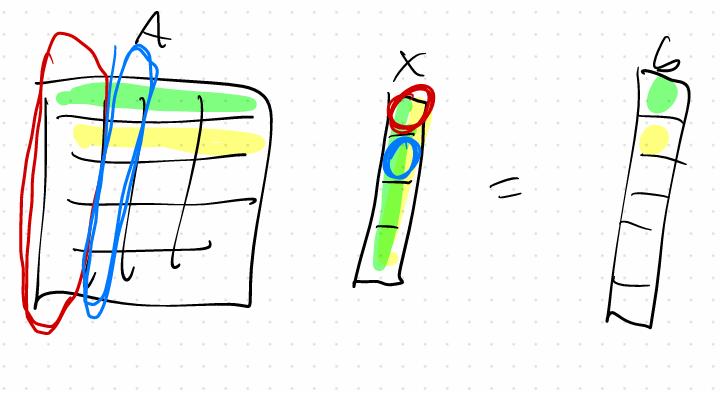
\includegraphics[width=0.75\linewidth]{Images/span.png}
    \caption{Span}
\end{figure}

\defn{Column Space of A}{
    Ax=b has only a solution, if b is in the span of the columns of A.
    This is called the column space of A or the range of A. Since this has to hold for each 
    vector b, and b is of dimensions 
    mx1, this implies that A 
    (dimensions mxn) must have at 
    least m columns, i.e., n>=m.
}

\defn{Rank}{
    The dimension of the column space is called the rank of the matrix.
}

\begin{figure}[H]
    \centering
    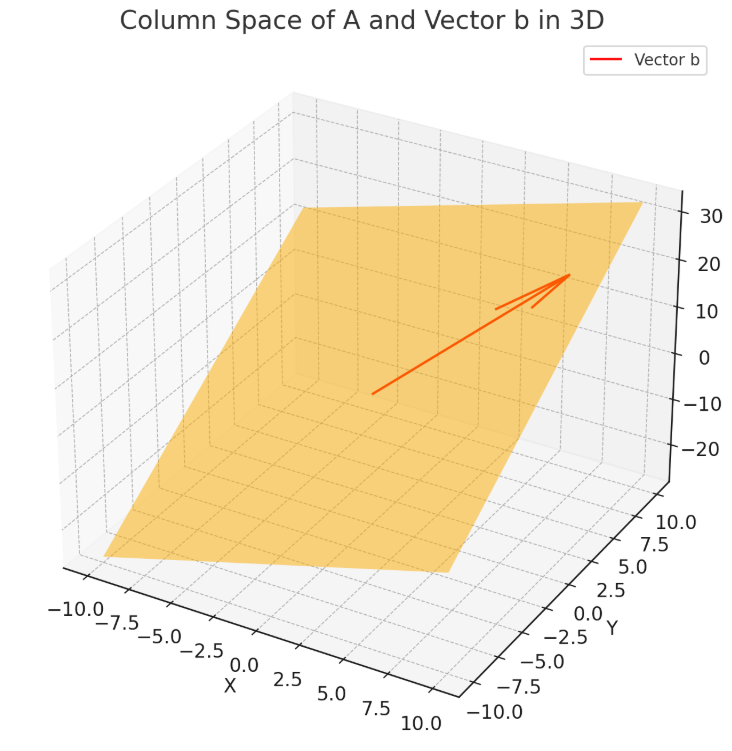
\includegraphics[width=0.5\linewidth]{Images/col-space-1.png}
    \caption{The 3D visualization of the column space of A,
    with the plane showing the span of the columns of A,
    and the red vector representing b. 
    If b b lies in this plane, it is in the column space, meaning a solution exists.an}
\end{figure}
\begin{figure}[H]
    \centering
    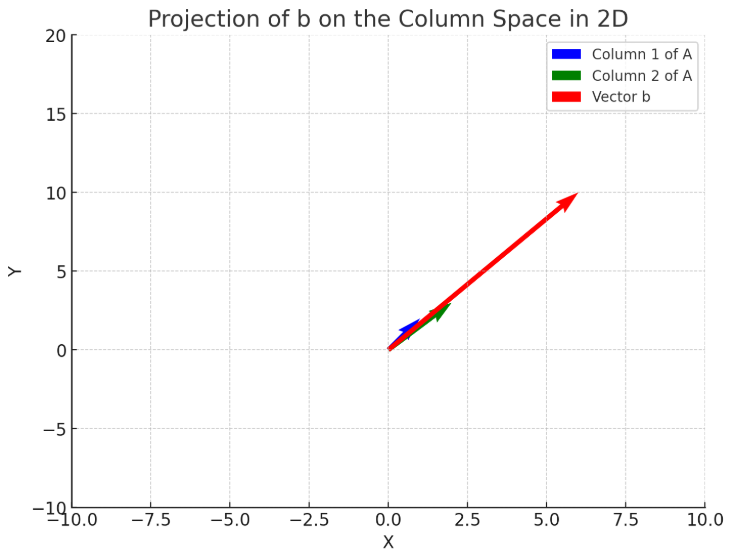
\includegraphics[width=0.5\linewidth]{Images/col-space-2.png}
    \caption{A 2D projection of the column space, showing how vector 
    b can be decomposed in terms of the two columns of A.
    If b lies within the span of these columns (the plane), a solution can be found.}
\end{figure}

\defn{Linear Independence}{
    Vector spaces, a set of vectors is said to be linearly independent if there exists
    no nontrivial linear combination of the vectors that equals the zero vector.
    If such a linear combination exists, then the vectors are said to be linearly dependent.
    \begin{equation}
        a_1 v_1 + a_2 v_2 + \cdots + a_k v_k = 0
    \end{equation}
    With at least one of the scalars is nonzero.

    Or with other words:
    A set of vectors is linearly 
    independent, if no vector in the set is 
    a linear combination of the other 
    vectors
}

\subsection{Norms}
\defn{Norm}{
    A norm is a way to measure the length of a vector.

    \begin{equation}
        \begin{split}
            f(x) &= 0 \Rightarrow x = 0 \\
            f(x+y) &\leq f(x) + f(y) \text{ triangle inequality} \\
            \forall \alpha \in \mathbb{R}, f(\alpha x) &= |\alpha| f(x)
        \end{split}
    \end{equation}
}

\defn{\(L^p\) Norm}{
    The euclidian norm is the \(L^p\) norm with p=2.
    \begin{equation}
        ||x||_p = (\sum_i |x_i|^p)^{\frac{1}{p}} \text{ for } p \in \mathbb{R},p \geq 1
    \end{equation}

    \begin{equation}
        ||x||_1 = \sum_{i} |x_i|
    \end{equation}

    \begin{equation}
        ||x||^2 = x^T x
    \end{equation}

    \begin{itemize}
        \item Close to zero, the squared norm increases very slowly
    \end{itemize}
}

\defn{Max Norm}{
    \(L^{\infty}\) norm which simplifies:
    \begin{equation}
        \begin{split}
            ||x||_{\infty} = \underset{i}{max} |x_i|
        \end{split}
    \end{equation}
}

\defn{Frobenius Norm}{
    Measures the size of a matrix, in a similar manner as the \(L^2\).
    \begin{equation}
        ||\boldsymbol{A}||_F = \sqrt{\sum_{i,j} A^2_{i,j}}
    \end{equation}
    \begin{equation}
        ||\boldsymbol{A}||_F = \sqrt{Tr(\boldsymbol{A}\boldsymbol{A}^T)}
    \end{equation}
}

\defn{Broadcasting}{
    In Deep Learning, it is common to 
    add scalars to matrices, which 
    means, that the scalar is added at 
    every entry of the matrix.
    \begin{equation}
        D = a \boldsymbol{B} + c
    \end{equation}

    It is further common to add 
    vectors to matrices, which means 
    that the vector is added to every 
    column of the matrix
    \begin{equation}
        \boldsymbol{C} = \boldsymbol{A} + \boldsymbol{b} \text{ where } C_{i,j} = A_{i,j} + b_j
    \end{equation}
}

\subsection{Matrix Decompositions}

\defn{Eigenvector}{
    a non-zero vector \textbf{v} that satisfies the eigen-equation is called an 
    eigenvector of \textbf{A} and the scalar \(\lambda\) 
    the corresponding eigenvalue:
    \begin{equation}
        \boldsymbol{Av} = \lambda \boldsymbol{v}
    \end{equation}

    This equation implies that any vector 
    \textbf{v} that is transformed by matrix \textbf{A} into 
    itself (except a scaling factor \(\lambda\)) is an 
    eigenvector of A. Hence the word 
    "Eigen", since the vector stays itself.
}

\defn{Eigendecomposition}{
    Decomposing a matrix into a set of eigenvectors and eigenvalues.
    \textbf{Focus on real symmetric matrices.}

    Assume that \textbf{A} has n linearly 
    independent eigenvectors and 
    corresponding eigenvalues
    Now we can concatenate these 
    eigenvectors to form a matrix \textbf{V} 
    and concatenate the 
    corresponding eigenvalues to 
    form the vector \(\lambda\):
    \begin{equation}
        \begin{split}
            \boldsymbol{V} &= [\boldsymbol{v}^{(1),} \cdots, \boldsymbol{v}^{(n)}] \\
            \boldsymbol{A} &= \boldsymbol{V} diag(\boldsymbol{\lambda}) \boldsymbol{V}^{-1}
        \end{split}
    \end{equation}

    \textbf{Every real and symmetric matrix has a eigendecomposition!}
    The eigenvectors are guaranteed to be orthogonal.
    \begin{equation}
        \boldsymbol{A} = \boldsymbol{Q\Lambda} \boldsymbol{Q}^T
    \end{equation}
    Because \textbf{Q} is orthogonal we can write \(\boldsymbol{Q}^T\) instead of \(\boldsymbol{Q}^{-1}\)
}

\begin{figure}[H]
    \centering
    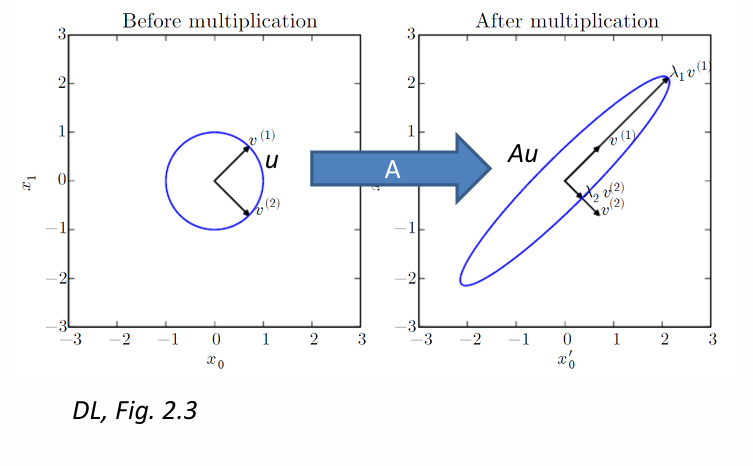
\includegraphics[width=0.75\linewidth]{Images/eigendecomp.png}
    \caption{Eigendecomposition, Blue Circle = All possible points reached using unit vectors,
    We then apply matrix \textbf{A} to each point. Eigenvectors are just scaled by the transformation by a eigenvalue}
\end{figure}

\defn{Eigendecomposition in Optimization}{
    For:
    \begin{equation}
        f(\boldsymbol{x}) = \boldsymbol{x}^T \boldsymbol{Ax} \text{ subject to } ||\boldsymbol{x}||_2 = 1
    \end{equation}
    If x is a unit eigenvector of A, then:
    \begin{equation}
        \begin{split}
            \boldsymbol{Ax} &= \lambda \boldsymbol{x} \\
            \boldsymbol{x}^T \boldsymbol{Ax} &= \boldsymbol{x}^T \lambda \boldsymbol{x} \\
            &= \lambda
        \end{split}
    \end{equation}
    \begin{itemize}
        \item The maximum of this function is now 
        found for the vector x corresponding 
        to the eigenvector belonging to the 
        maximum eigenvalue.
        \item Similarly, the minimum of the 
        function f(x) is the eigenvector 
        belonging to the minimum 
        eigenvalue.
    \end{itemize}
}

\defn{Singular Value Decomposition (SVD)}{
    Is a more general way of factoring a matrix into singular vectors and values.
    Every real matrix has an SVD.
    \begin{equation}
        \boldsymbol{A} = \boldsymbol{UD} \boldsymbol{V}^T
    \end{equation}
    \begin{description}
        \item[A] mxn Matrix
        \item[U] An orthogonal mxm matrix. Cols are called left-singular vectors, these are eigenvectors of \(AA^T\).
        \item[D] Diagonal mxn matrix. The diagonal elements are called singular values. Non-zero sv are square roots of eigenvalues of \(AA^T\).
        \item[V] Orthogonal nxn matrix. Cols are called right-singular vectort and are eigenvectors of \(A^T A\)   
    \end{description}
}
\subsection{Pseudoinverse}
The inverse of a matrix is undefined if its not square.
This means that the inverse is of little use in deep learning.
What we really want is in a underdefined or overdefined problem to find the best fitting solution.
\defn{Moore-Penrose Pseudoinverse}{
    The Moore-Penrose 
    pseudoinverse allows for a 
    reasonable solution in both cases (under or overdefined)
    and is defined as a limit.
    \begin{equation}
        \begin{split}
            \boldsymbol{A}^+ &= \lim_{a\searrow 0}( \boldsymbol{A}^T  \boldsymbol{A} + \alpha  \boldsymbol{I})^{-1}  \boldsymbol{A}^T \\
            \boldsymbol{A}^+ &=  \boldsymbol{V}  \boldsymbol{D}^+  \boldsymbol{U}^T
        \end{split}
    \end{equation}

    Note the similarity to the SVD, 
    basically the pseudoinverse is the 
    transpose of A=UDVT, which 
    would result in AT=VDTUT
    The transpose is simply the 
    inverse for orthogonal matrixes 
    (U and V) but not for D. With:
    \begin{equation}
        D^+_{i,j} = 1/D^+_{i,j}
    \end{equation}

    \begin{equation}
        \boldsymbol{A}^+ \boldsymbol{A} = \boldsymbol{I}
    \end{equation}

    \begin{itemize}
        \item When there are more unknowns 
        (columns n) than equations (rows 
        m), then the pseudoinverse 
        returns the shortest vector 
        \(x=A^+y\), among all possible 
        solutions.
        \begin{equation*}
            \boldsymbol{x} = \boldsymbol{A}^+\boldsymbol{y} \text{ with minimal } ||\boldsymbol{x}||_2
        \end{equation*}
        \item When there are more equations 
        (rows m) than unknowns 
        (columns n), then the 
        pseudoinverse returns the vector 
        x such that Ax is as close as 
        possible to the vector y
        \begin{itemize}
            \item RSS/MSE optimal solution
        \end{itemize}
        \begin{equation*}
            \begin{split}
                \boldsymbol{Ax} &= \boldsymbol{y} \\
                \Rightarrow &min(||\boldsymbol{Ax} - \boldsymbol{y}||_2)
            \end{split}
        \end{equation*}
    \end{itemize}
}

\subsection{Trace and Determinant}

\defn{Trace}{
    \begin{equation}
        Tr(\boldsymbol{A}) = \sum_{i} A_{i,i}
    \end{equation}
    Used to replace a sum over some squared errors.
    \begin{equation*}
        ||\boldsymbol{A}||_F = \sqrt{Tr(\boldsymbol{A}\boldsymbol{A}^T)}
    \end{equation*}

    \begin{equation}
        \begin{split}
            Tr(\boldsymbol{A}^T) &= Tr(\boldsymbol{A}) \\
            Tr(\boldsymbol{AB}) &= Tr(\boldsymbol{BA}) \\
            Tr(\boldsymbol{ABC}) &= Tr(\boldsymbol{CAB}) = Tr(\boldsymbol{BCA}) \\
            Tr(A) &= \sum_{i} \lambda_i
        \end{split}
    \end{equation}
    The trace is the sum of all eigenvalues.
}

\defn{Determinant}{
    \begin{equation}
        det(\boldsymbol{A}) = \prod_{i} \lambda_i
    \end{equation}
}


\begin{figure}[H]
    \centering
    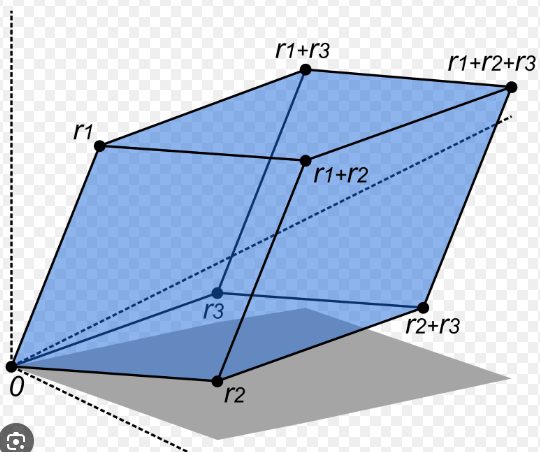
\includegraphics[width=0.5\linewidth]{Images/determinant.png}
    \caption{In 3D space the determinant shows the change in volume after the transformation. (in 2D the area)}
\end{figure}

\section{Ergänzungen DMI}
\begin{figure}[H]
    \centering
    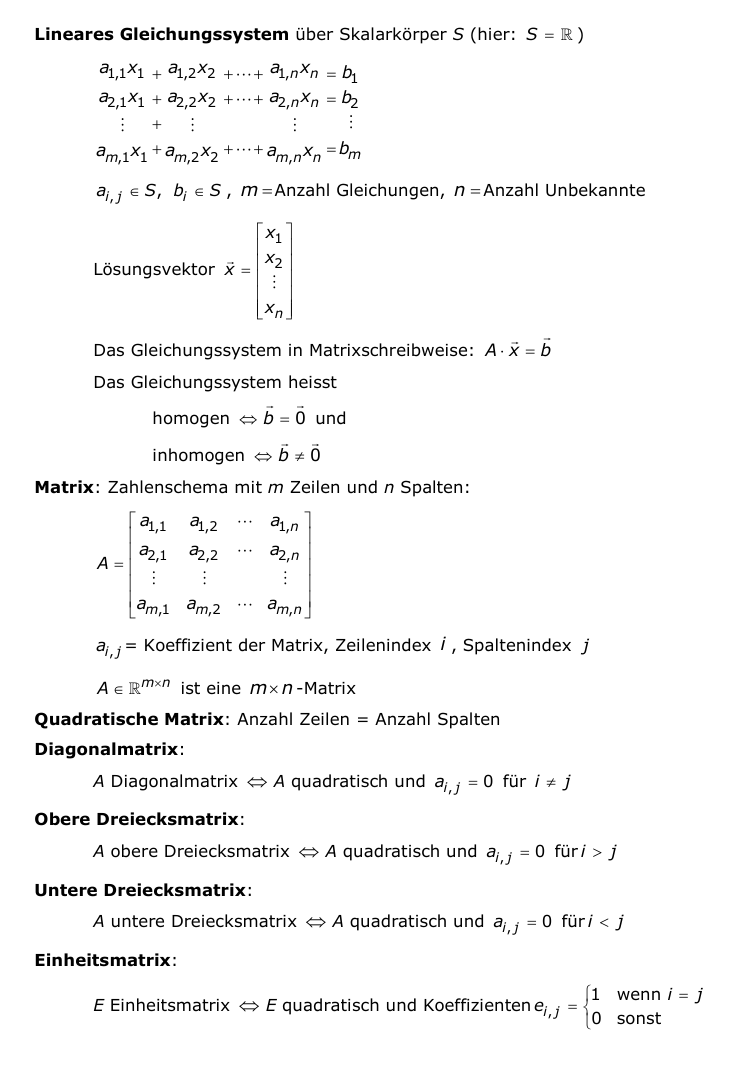
\includegraphics[width=0.75\linewidth]{Images/dmi_1.png}
    \caption{LinAlg Zusammenfassung 1}
\end{figure}

\begin{figure}[H]
    \centering
    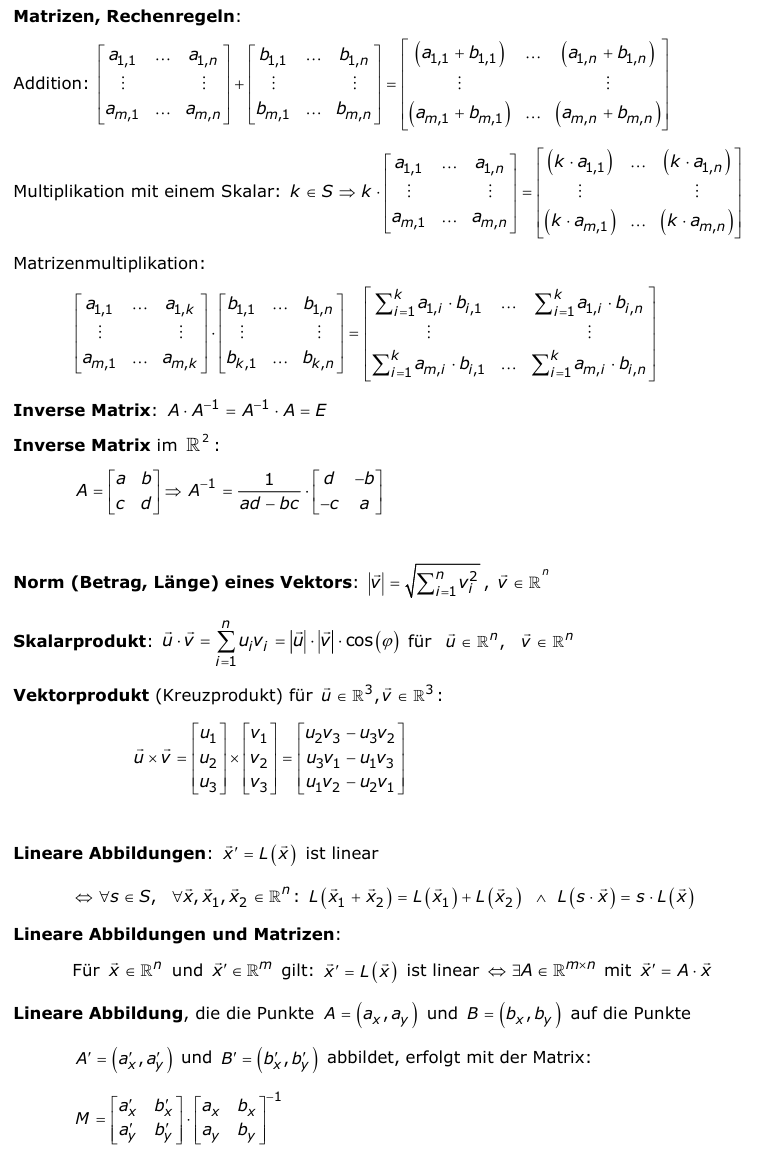
\includegraphics[width=0.75\linewidth]{Images/dmi_2.png}
    \caption{LinAlg Zusammenfassung 2}
\end{figure}

\begin{figure}[H]
    \centering
    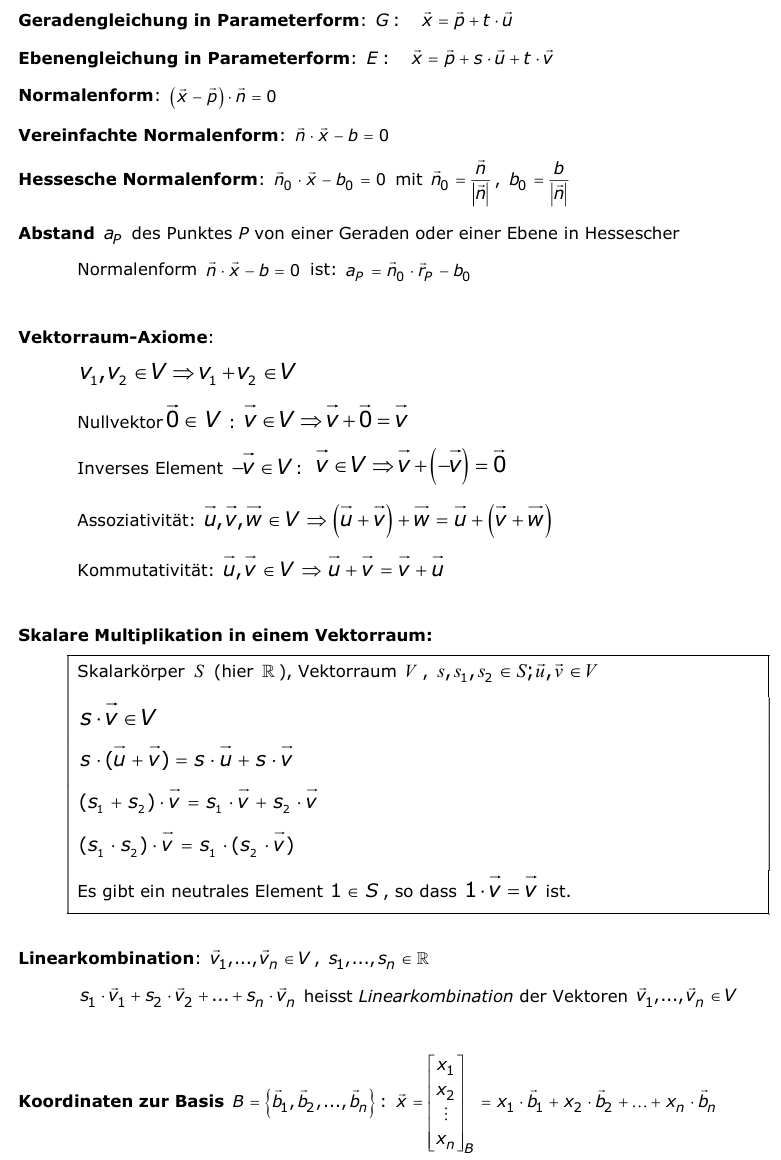
\includegraphics[width=0.75\linewidth]{Images/dmi_3.png}
    \caption{LinAlg Zusammenfassung 3}
\end{figure}

\begin{figure}[H]
    \centering
    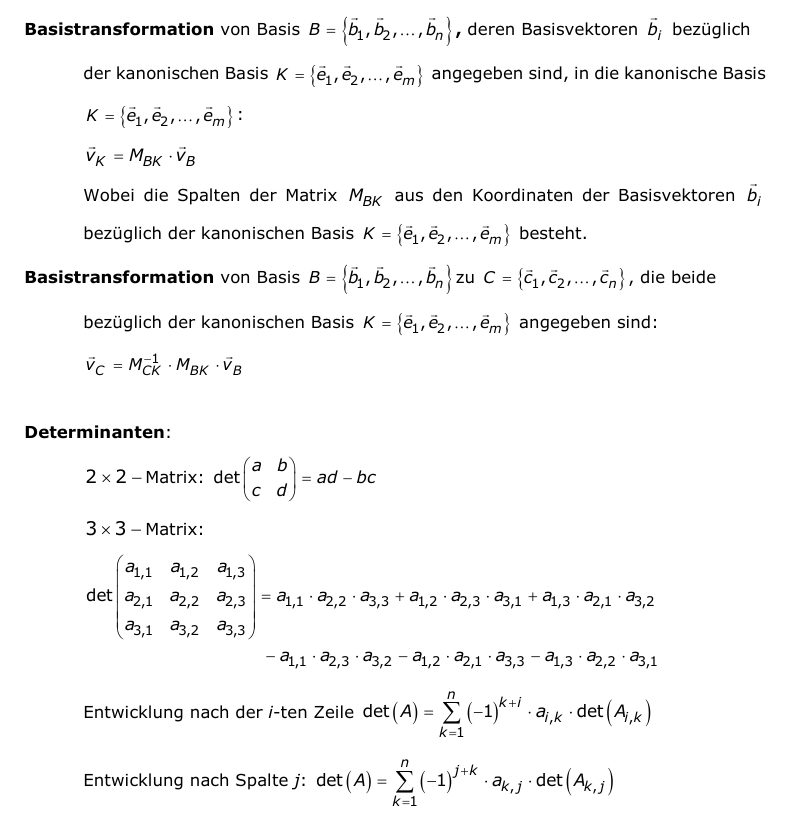
\includegraphics[width=0.75\linewidth]{Images/dmi_4.png}
    \caption{LinAlg Zusammenfassung 4}
\end{figure}

\section{Ergänzungen Wahrscheinlichkeiten}

\subsection{Sources of uncertainty}
\begin{itemize}
    \item Inherent stochasticity in the system being modeled
    \item Incomplete observaboöoty
    \item Incomplete modeling
\end{itemize}

\subsection{Recap}

\defn{Discrete Random Variables - Probability Mass Functions (PMF)}{
    \begin{equation}
        \begin{split}
            X \sim P(X) \\
            \text{Domain of } P(X) = \text{ all possible states} \\
            0 \leq P(x) \leq 1 \\
            \sum P(X) = 1
        \end{split}
    \end{equation}
    Note that probability 0 is not impossible as 
    stated on the right but improbable vice versa for 1.
}

\defn{Continues Random Variables - Probability Density Functions}{
    In englisch we explicitly differentiate with using the term "density"
    or even better "likelyhood".
    \begin{equation}
        \begin{split}
            X \sim p(X) \\
            \text{Domain of } P(X) = \text{ all possible values} \\
            0 \leq P(x) \\
            \int P(X) = 1 \\
            P(a \leq x \leq b) = \int_{a}^{b} p(x) dx
        \end{split}
    \end{equation}
}

\defn{Uniform PDF}{
    \begin{equation}
        X \sim U(a,b) = \frac{1}{b-a}
    \end{equation}
}

\defn{Marginalization}{
    Simply sum (integrate) over all 
    variables one is not interested in. These distributions are then called 
    marginal probability distributions, 
    but they are just pmf/pdf of the particular rv.
    \begin{equation}
        \begin{split}
            \forall x \in X, P(X=x) = \sum_{y} P(X=x, Y=y) \\
            p(x) = \int p(x,y) dy
        \end{split} 
    \end{equation}
}

\defn{Conditional Probability}{
    \begin{equation}
        P(Y=y | X=x)= \frac{P(Y=y, X=x)}{P(X=x)}
    \end{equation}
    Or use Bayes!
    \begin{equation}
        \begin{split}
            P(X|Y) = \frac{P(X)}{P(Y)} P(Y|X) \\
            P(Y) = \sum_{X} P(Y|X) P(X)
        \end{split}
    \end{equation}
    Note:
    \begin{equation*}
        P(x|y)P(y)=P(x,y)=P(y,x)=P(y|x)P(x)
    \end{equation*}
}

\begin{figure}[H]
    \centering
    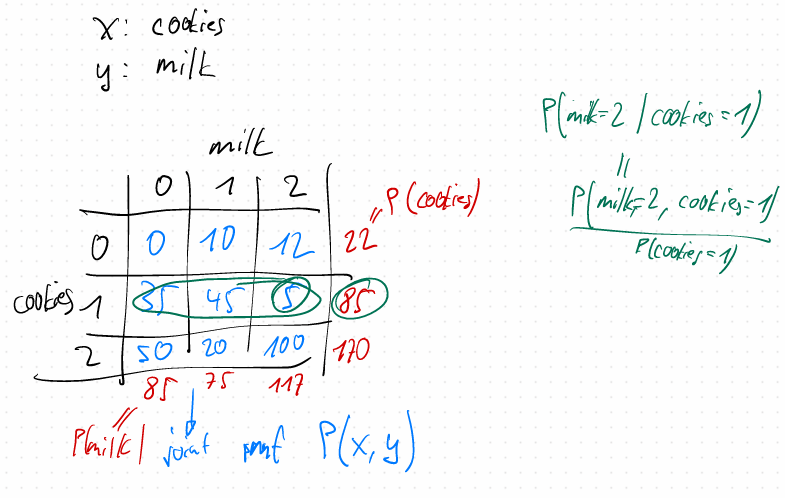
\includegraphics[width=0.5\linewidth]{Images/jointprob.png}
    \caption{Marginalization}
\end{figure}

\defn{Chain Rule of Conditional Probabilities}{
    \begin{equation}
        P(x^{(1)},\cdots,x^{(n)}) = P(x^{(1)}) \prod_{i=2}^{n} P(x^{(i)} | x^{(1)},\cdots,x^{(i-1)})
    \end{equation}
    This follows from:
    \begin{equation*}
        \begin{split}
            P(Y=y | X=x) &= \frac{P(Y=y, X=x)}{P(X=x)} \\
            \Rightarrow \\
            P(a,b,c) &= P(a|b,c)P(b,c) \\
            P(b,c) &= P(b|c)P(c) \\
            P(a,b,c) &= P(a|b,c)P(b|c)P(c)
        \end{split}
    \end{equation*}
}

\defn{Statistical Independence}{
    \begin{equation}
        \begin{split}
            \forall x \in X, y \in Y, p(X=x,Y=y) = p(X=x)p(Y=y)\\
            = x \perp y
        \end{split}
    \end{equation}
    This also applies for conditionals:
    \begin{equation}
        \begin{split}
            x \perp y | z \\
            = p(X=x | Z=z) p(Y=y | Z=z)
        \end{split}
    \end{equation}
}

\defn{Different Notation for Excpectation}{
    \begin{equation}
        \begin{split}
            \mathop{\mathbb{E}}_{x \sim P}[f(x)] &= \sum_{x} P(x)f(x) \\
            \mathop{\mathbb{E}}_{x \sim p}[f(x)] &= \int p(x) f(x) dx
        \end{split}
    \end{equation}
    With simplified notation:
    \begin{equation}
        \begin{split}
            \mathop{\mathbb{E}}_x[f(x)]\\
            \mathop{\mathbb{E}}[f(x)]
        \end{split}
    \end{equation}
    \begin{itemize}
        \item Expectation is a linear operator
    \end{itemize}
}

\defn{Different Notation for Variance}{
    The variance measures the expected 
    squared distance of f(x) to its 
    expected value E[f(x)].
    \begin{equation}
        Var(f(x)) = \mathop{\mathbb{E}}[(f(x)-\mathop{\mathbb{E}}[f(x)])^2]
    \end{equation}
}

\defn{Different Notation for Covariance}{
    Gives some insights 
    of how much two rvs are linearly 
    related to each other and also 
    the scale of these rvs.

    \begin{equation}
        Cov(f(x),g(x)) = \mathop{\mathbb{E}}[(f(x)- \mathop{\mathbb{E}}[f(x)]) (g(y)-\mathop{\mathbb{E}}[g(y)])]
    \end{equation}

    The correlation is the covariance 
    divided by the standard deviations of 
    f(x) and f(y) and can only be in the 
    range of -1 to +1:
    \begin{equation}
        p_{X,Y} = corr(X,Y) = \frac{cov(X,Y)}{\sigma_X \sigma_Y}
    \end{equation}

    Independent rvs have a 
    covariance of 0 but a covariance 
    of 0 does not necessarily mean, 
    that the rvs are independent
}

\defn{Covariance Matric}{
    Of a random vector \(\boldsymbol{x} \in R^n\) is a nxn matrix, such that:
    \begin{equation}
        Cov(x)_{i,j} = Cov(x_i, x_j)
    \end{equation}
    The diagonal elements give the variance:
    \begin{equation}
        Cov(x_i, x_i) = Var(x_i)
    \end{equation}
}

\begin{figure}[H]
    \centering
    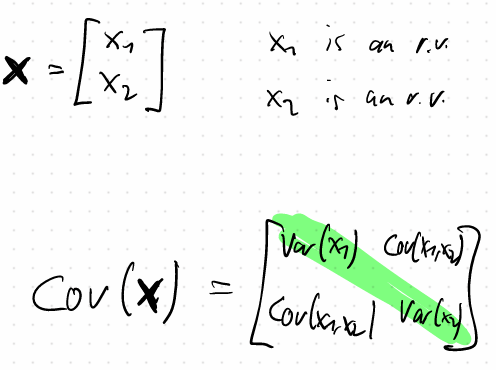
\includegraphics[width=0.5\linewidth]{Images/covmatrix.png}
    \caption{Covariance Matrix}
\end{figure}

\section{Further Distributions}
\defn{Bernoulli}{
    \begin{equation}
        \begin{split}
            P(x=1) = \phi \\
            P(x=0) = 1- \phi \\
            \mathop{\mathbb{E}}[x] = \phi \\
            Var(x) = \phi(1-\phi)
        \end{split}
    \end{equation}
}

\begin{figure}[H]
    \centering
    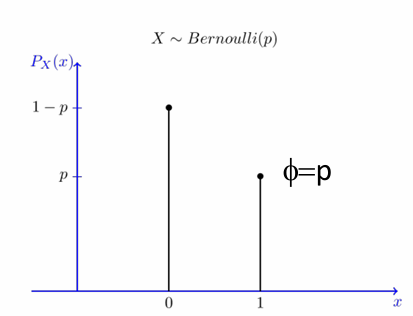
\includegraphics[width=0.5\linewidth]{Images/bernoulli-d.png}
    \caption{Bernoulli Distribution}
\end{figure}

\defn{Multinoulli}{
    Distribution over a discrete variable with k states \(p \in [0,1]^{k-1}\).
    \textbf{p} is a vector with k-1 elements, where each entry \(p_i\) is the probability of state i.

    The final states probability 
    \(p_k\) is given by:
    \begin{equation}
        p_k = 1-\boldsymbol{1}^T \boldsymbol{p}
    \end{equation}

    Used to describe probabilities over a finite number of classes.
}

\defn{Gaussian}{
    \begin{equation}
        N(x; \mu, \sigma^2) = \sqrt{\frac{1}{2 \pi \sigma^2}} exp(-\frac{1}{2\sigma^2} (x-\mu)^2)
    \end{equation}
    Alternative parameterization, where \(\beta\) is called the precision:
    \begin{equation}
        N(x; \mu, \beta^{-1}) = \sqrt{\frac{\beta}{2 \pi}} exp(-\frac{1}{2}\beta (x-\mu)^2)
    \end{equation}
    \(\beta\) is simply \(\frac{1}{\sigma^2}\)


    \begin{itemize}
        \item central limit theorem, which 
        states that the sum of many 
        independent rvs approaches a 
        Gaussian distribution
        \item For a given variance, the Gaussian 
        distribution has the largest 
        uncertainty (differential entropy) 
    \end{itemize}
    \begin{equation*}
        h(X) = - \int_{X} f(x) log f(x) dx
    \end{equation*}
    An in multiple dimensions:
    \begin{equation}
        N(x; \mu, \Sigma) = \sqrt{\frac{1}{(2 \pi)^n det(\Sigma)}} exp(-\frac{1}{2}(x-\mu)^T \Sigma^{-1} (x-\mu)^2)
    \end{equation}
    \begin{equation}
        N(x; \mu, \beta^{-1}) = \sqrt{\frac{det(\beta)}{(2 \pi)^n }} exp(-\frac{1}{2}(x-\mu)^T \beta (x-\mu)^2)
    \end{equation}
    \begin{itemize}
        \item For simplicity, the covariance matrix 
        is often assumed to be a diagonal 
        matrix, hence all dimensions of x are 
        uncorrelated
        \item An even simpler model is the 
        isotropic Gaussian distribution since 
        the covariance matrix is simply a 
        scalar times the identity matrix. 
        Hence the dimensions are not only 
        uncorrelated but also all have the 
        same variance.
    \end{itemize}
}

\begin{figure}[H]
    \centering
    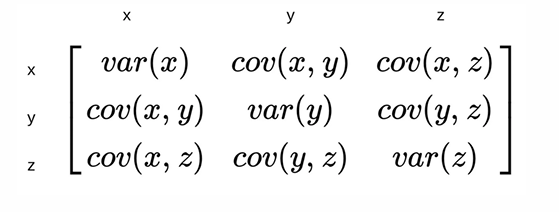
\includegraphics[width=0.5\linewidth]{Images/covmatrix2.png}
    \caption{Example Covmatrix}
\end{figure}

\begin{figure}[H]
    \centering
    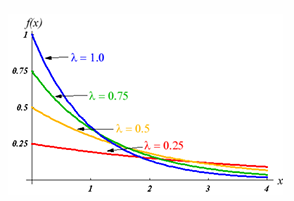
\includegraphics[width=0.5\linewidth]{Images/1func.png}
    \caption{\(\boldsymbol{1}_{x\geq0}\) Function}
\end{figure}

\defn{Exp and Laplace Distribution}{
    \begin{equation}
        p(x;\lambda) = \lambda \boldsymbol{1}_{x \geq 0} exp(- \lambda x)
    \end{equation}
    \begin{itemize}
        \item 1 if the 
        argument (.) is greater or equal zero 
        and zero otherwise.
        \item In other words, for negative values of 
        x, the exponential function is zero
        \item The larger \(\lambda\), the more extreme is the 
        peak at zero
    \end{itemize}

    If the peak should be at an 
    arbitrary point, then the Laplace 
    distribution is helpful:
    \begin{equation}
        Laplace(x; \mu, \gamma) = \frac{1}{2\gamma} exp(- \frac{|x - \mu|}{\gamma})
    \end{equation}
}

\begin{figure}[H]
    \centering
    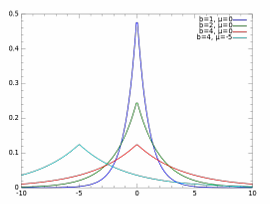
\includegraphics[width=0.5\linewidth]{Images/laplace-d.png}
    \caption{Laplace Distribution: The bigger \(gamma\), the steeper the peek, peak is at \(\mu\)}
\end{figure}

\defn{Dirac}{
    Using a Dirac delta function, it is 
    possible to define pdfs which 
    have a probability greater than 
    zero at one given point.
    \begin{equation}
        p(x) = \delta(x - \mu)
    \end{equation}
}

\begin{figure}[H]
    \centering
    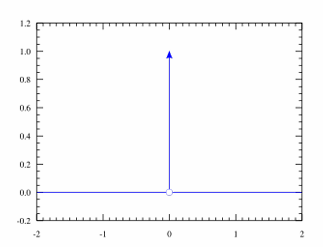
\includegraphics[width=0.5\linewidth]{Images/dirac.png}
    \caption{Dirac Distribution: Arrows shows the functions goes to \(\infty\)}
\end{figure}

\defn{Empirical Distribution}{
    Using dirac delta we can describe density functions using discrete data.
    \textbf{The function is 0 everywhere, except at 0, there it goes to infinity.}
    \begin{equation}
        \hat{p}(\boldsymbol{x}) = \frac{1}{m} \sum_{i=1}^{m} \delta(\boldsymbol{x}-\boldsymbol{x}^{(i)})
    \end{equation}
}

\section{Common Functions}
\defn{Sigmoid}{
    De-Facto standard in binary classification:
    \begin{equation}
        \sigma(x) = \frac{1}{1+ exp(-x)}
    \end{equation}
    \begin{itemize}
        \item Note that for very small and very 
        large value of x, the sigmoid saturates 
        to 0 respectively 1 and the 
        derivatives at those values converge 
        towards 0. This will become a problem later on
    \end{itemize}
}

\begin{figure}[H]
    \centering
    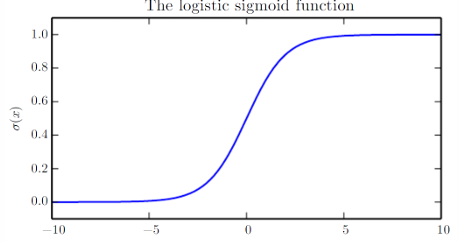
\includegraphics[width=0.5\linewidth]{Images/sigmoid.png}
    \caption{Sigmoid Function}
\end{figure}

\begin{figure}[H]
    \centering
    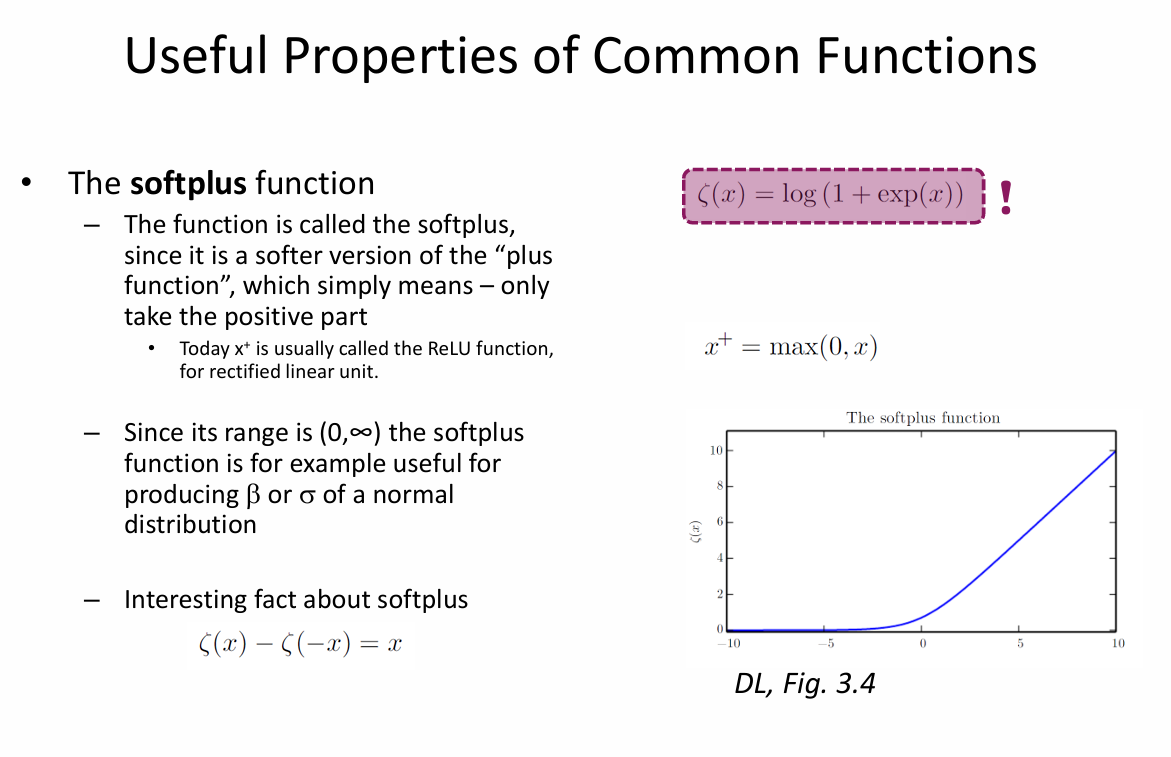
\includegraphics[width=1\linewidth]{Images/relu.png}
    \caption{RELU Function}
\end{figure}

\begin{figure}[H]
    \centering
    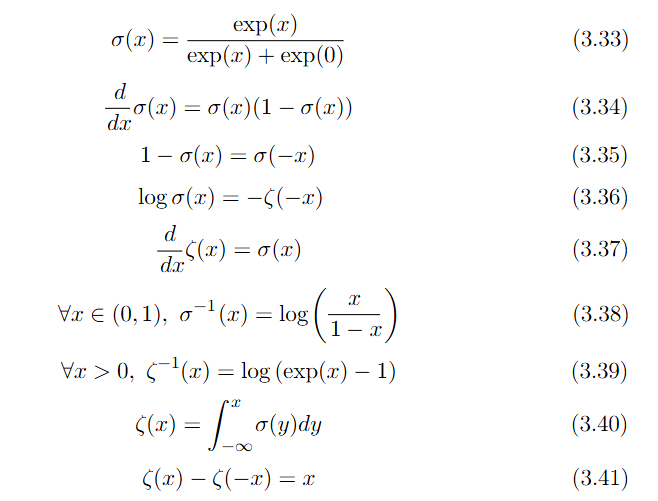
\includegraphics[width=1\linewidth]{Images/comm-useful-props.png}
    \caption{Useful Properties ofCommon Functions}
\end{figure}

\section{Introduction}

\begin{figure}[H]
    \centering
    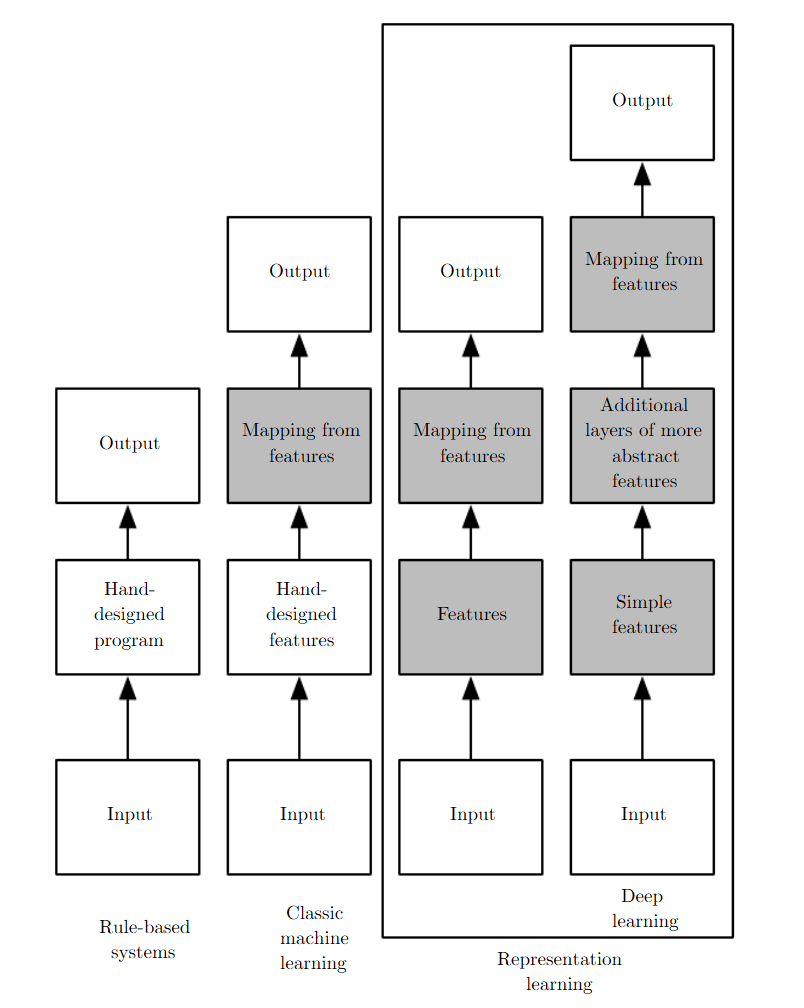
\includegraphics[width=0.75\linewidth]{Images/deepl-diff.png}
    \caption{Flowcharts showing the relation between different parts of an AI system}
\end{figure}
\defn{Knowledge Encoding}{
    Several artificial intelligence projects have sought to hard-code knowledge about
    the world in formal languages. A computer can reason automatically about statements
    in these formal languages using logical inference rules. This is known as the knowledge
    base approach to artificial intelligence. None of these projects has led to a major success.
    https://www.deeplearningbook.org/contents/intro.html
}

The diffculties faced by systems relying on hard-coded knowledge suggestthat AI systems 
need the ability to acquire their own knowledge, by extracting
patterns from raw data. This capability is known as machine learning.
The performance of these simple machine learning algorithms depends heavily
on the representation of the data they are given. (Example: Graph using Caresian vs Polar coordinates)


One solution to this problem is to use machine learning to discover not only
the mapping from representation to output but also the representation itself.
This approach is known as representation learning.
The quintessential example of a representation learning algorithm is the \textbf{autoencoder}.

\defn{Feature Design}{
    When designing features or algorithms for learning features, our goal is usually
    to separate the factors of variation that explain the observed data.

    The word "factors" simply to refer to separate sources of influence
}

When it is nearly as diffcult to obtain a representation as to solve theoriginal problem,
representation learning does not, at first glance, seem to help us.

\textbf{Deep learning} solves this central problem in representation learning by 
introducing representations that are expressed in terms of other, simpler representations.

\defn{Perspectives of Deep Learning}{
    The idea of learning the right representation for the data provides one perspective on deep learning.
    (Encodes factors of variation that explain the input)
    Another perspective on deep learning is that depth
    enables the computer to learn a multistep computer program.
}

\begin{figure}[H]
    \centering
    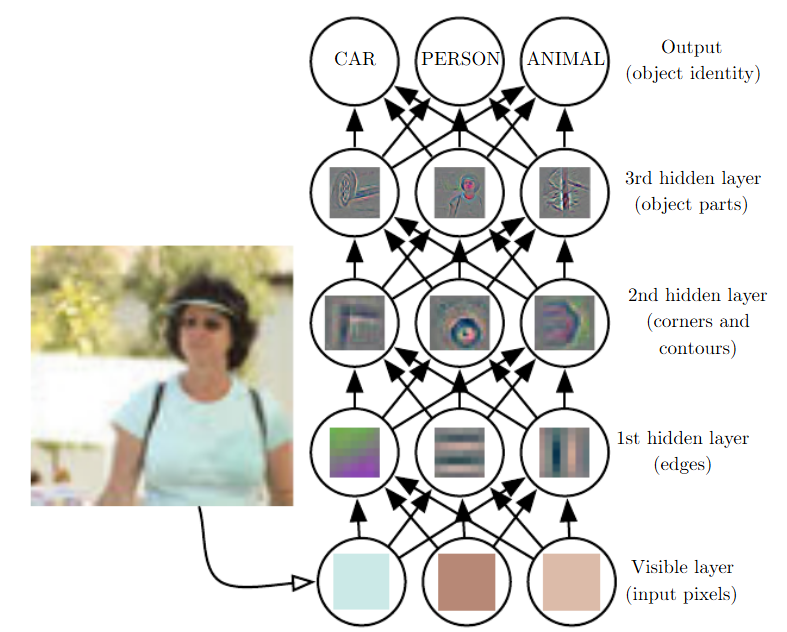
\includegraphics[width=0.75\linewidth]{Images/multistepalgorithm.png}
    \caption{An alorithm breaks a problem into feasable subproblems. It itself learns the data's representation.}
\end{figure}

\begin{figure}[H]
    \centering
    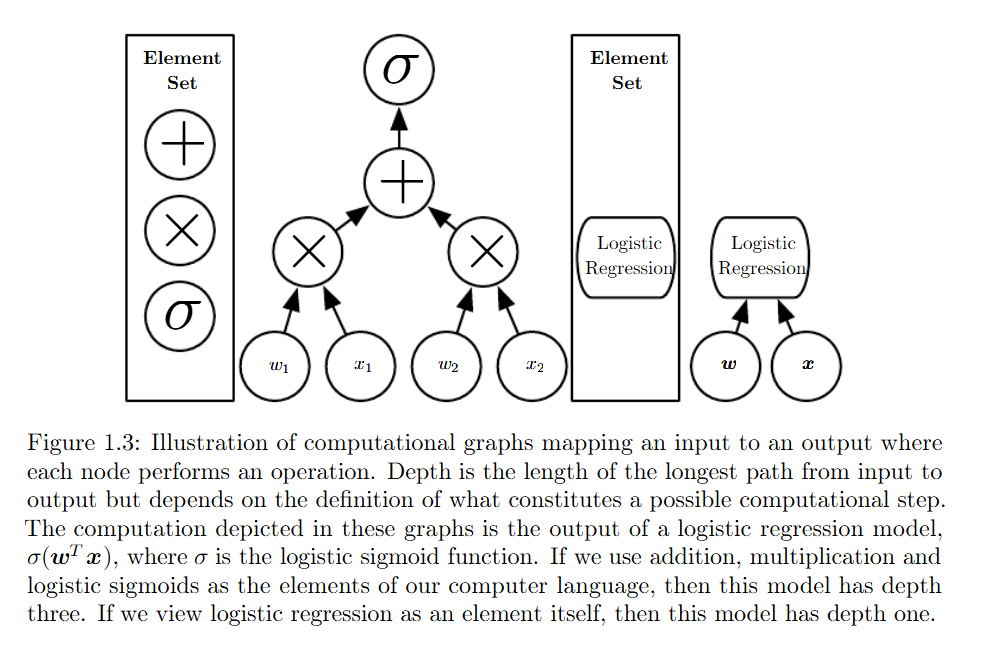
\includegraphics[width=0.75\linewidth]{Images/computational-depth.png}
\end{figure}

Deep learning can be safely regarded as thestudy of models that involve a greater amount of composition 
of either learned functions or learned concepts than traditional machine learning does.

\end{document}
